% 原印刷87--104页／PDF物理113--130，止于§3.2标题之前.
\autoref{sec:1}在基于对偶方法的最优传输一般理论框架内，对形如$c(x,y)=h(x-y)$且$h$严格凸的成本，给出了最优传输映射的存在性结果. 特别地，取$c(x,y)=|x-y|^p$，这一结果适用于$p\in]1,+\infty[$时的极小化问题
\[
\min\{\|\mathrm T-\mathrm{id}\|_{L^p(\mu)}:\mathrm T_\#\mu=\nu\}
\]
（用Kantorovich语言表示为$\min\{\|y-x\|_{L^p(\gamma)}:\gamma\in\Pi(\mu,\nu)\}$）. 本章考察两个极限情形$p=1$与$p=\infty$，它们需要额外技巧.

随后，讨论部分沿两个不同方向展开：一方面，$L^1$与$L^\infty$情形引出了对于可能不严格凸、或在某些地方取无穷值的凸成本的研究，\autoref{sec:3.3.1}将讨论这一主题的最新进展；另一方面，人们也会问$0<p<1$时情况如何，更一般地，关于距离为递增凹函数的成本又如何，这将是\autoref{sec:3.3.2}的主题.

\subsection[成本为距离的Monge情形]{Monge情形：成本为$|x-y|$}\label{sec:3.1}
本节将证明：若$\mu,\nu\in\mathscr P(\Omega)$，其中$\Omega\subset\mathbb R^d$为紧区域，且$\mu\ll\mathscr L^d$，则成本$|x-y|$（$\mathbb R^d$中的欧氏距离）存在最优传输映射$\mathrm T$. 我们给出的证明主要归于Ambrosio\cite{b8}，它是对Sudakov证明\cite{b290}的修改. 导论已经给出这一情形下其他存在性证明的参考文献.

\subsubsection{距离成本的对偶性}\label{sec:3.1.1}
先讨论成本$c(x,y)$本身就是距离的情形（因而满足三角不等式，当$x=y$时为零，等等）. 由于成本对称，不再区分$\bar c$-变换与$c$-变换.

\begin{proposition}\label{obj:3.1}
若$c:X\times X\to\mathbb R$是距离，则函数$u:X\to\mathbb R$为$c$-凹函数，当且仅当它关于距离$c$为Lipschitz连续函数且Lipschitz常数小于$1$. 这些函数的集合记为$\operatorname{Lip}_1$. 此外，对每个$u\in\operatorname{Lip}_1$都有$u^c=-u$.
\end{proposition}

\begin{proof}
先取$c$-凹函数$u$. 对某个函数$\chi:X\to\mathbb R\cup\{-\infty\}$，可写成
\[
u(x)=\chi^c(x)=\inf_y c(x,y)-\chi(y).
\]
可忽略满足$\chi(y)=-\infty$的点$y$；对其余的点，注意$x\mapsto c(x,y)-\chi(y)$为$\operatorname{Lip}_1$函数，因为由三角不等式，$x\mapsto c(x,y)$为$\operatorname{Lip}_1$函数. 因而$u\in\operatorname{Lip}_1$，因为具有相同Lipschitz常数的一族Lipschitz连续函数的下确界仍具有相同的连续模.

现在取函数$u\in\operatorname{Lip}_1$. 我们断言可以写成
\[
u(x)=\inf_y c(x,y)+u(y).
\]
事实上，显然右侧下确界不大于$u(x)$，因为总可以取$y=x$. 另一方面，$u\in\operatorname{Lip}_1$意味着$u(x)-u(y)\le c(x,y)$，即对每个$y$都有$u(x)\le u(y)+c(x,y)$，因而下确界不小于$u(x)$. 这一表达式说明$u=(-u)^c$，故$u$为$c$-凹函数.

把最后一个公式应用于同样属于$\operatorname{Lip}_1$的$-u$，便得$u^c=-u$，陈述的最后部分随之得证.
\end{proof}

由此，当成本函数为距离时，对偶公式给出
\begin{equation}\label{eq:3.1}
\min\left\{\int_{X\times X}c(x,y)\,d\gamma:\gamma\in\Pi(\mu,\nu)\right\}
=\max\left\{\int_Xu\,d(\mu-\nu):u\in\operatorname{Lip}_1\right\}.
\end{equation}
这也蕴含距离成本$c$对应的传输代价$\mathscr T_c$的一个有用性质，即它满足三角不等式. 我们会在\autoref{sec:5}再次看到这一点：那里用$c(x,y)=|x-y|^p$对应的传输代价$\mathscr T_c$来定义$\mathscr P(\Omega)$上的距离. 在这里强调它，是因为本章稍后将要使用.

\begin{corollary}\label{obj:3.2}
若$c:X\times X\to\mathbb R$是距离，则给定$\mu,\nu,\varrho\in\mathscr P(X)$，有
\[
\mathscr T_c(\mu,\nu)\le\mathscr T_c(\mu,\varrho)+\mathscr T_c(\varrho,\nu).
\]
\end{corollary}
\begin{proof}
任取函数$u\in\operatorname{Lip}_1$，写成
\[
\int u\,d(\mu-\nu)=\int u\,d(\mu-\varrho)+\int u\,d(\varrho-\nu)
\le\mathscr T_c(\mu,\varrho)+\mathscr T_c(\varrho,\nu).
\]
对$u$取上确界即得结论.
\end{proof}

还要指出距离特有的另一个有用性质.
\begin{corollary}\label{obj:3.3}
若$c:X\times X\to\mathbb R$是距离，且$\mu,\nu$满足$\mathscr T_c(\mu,\nu)=0$，则$\mu=\nu$.
\end{corollary}
\begin{proof}
这一简单事实有多种证明. 例如，对偶公式给出对每个$u\in\operatorname{Lip}_1$都有$\int u\,d(\mu-\nu)=0$，这已足以保证$\mu=\nu$. 也可以直接注意到，$\mathscr T_c(\mu,\nu)=0$意味着存在$\gamma\in\Pi(\mu,\nu)$使$\int c\,d\gamma=0$，即$c(x,y)=0$在$\gamma$-几乎处处成立. 由于$c$是距离，这意味着$x=y$在$\gamma$-几乎处处成立，从而对每个检验函数$\phi$，都有$\int\phi\,d\mu=\int\phi(x)\,d\gamma=\int\phi(y)\,d\gamma=\int\phi\,d\nu$，因而$\mu=\nu$.
\end{proof}

\subsubsection{次级变分问题}\label{sec:3.1.2}
正如在搬书的\autoref{obj:2.15}中已经看到的，对于$\mathbb R$中$|x-y|$这样的距离成本，最优$\gamma$一般并不唯一. 现在希望选取一个特殊的最优解$\bar\gamma$，从而能够证明它由传输映射诱导. 为简单起见，由于很快要使用问题的一些欧氏特征，特别是它与二次成本$|x-y|^2$的联系，我们回到欧氏空间$\mathbb R^d$中的区域$\Omega$上的具体表述. 特别地，不再使用一般距离，而只使用欧氏范数.

以$O(\mu,\nu)$表示成本$|x-y|$的最优传输方案集合. 为固定记号，以$K_p$表示把$\gamma\in\mathscr P(\Omega\times\Omega)$对应到$\int|x-y|^p\,d\gamma$的泛函，并以$m_p$表示它在$\Pi(\mu,\nu)$上的最小值. 以此语言，
\[
O(\mu,\nu)=\operatorname*{argmin}_{\gamma\in\Pi(\mu,\nu)}K_1(\gamma)
=\{\gamma\in\Pi(\mu,\nu):K_1(\gamma)\le m_1\}.
\]
注意，$O(\mu,\nu)$是紧集$\Pi(\mu,\nu)$的一个闭子集（关于测度的弱收敛）. 只要极小化的是关于$\gamma$的下半连续泛函，这都是一般事实.

从现在起，固定从$\mu$到$\nu$、成本$c(x,y)=|x-y|$的传输的一个Kantorovich势$u$，并将其作为检验最优性的工具. 事实上，
\begin{equation}\label{eq:3.2}
\gamma\in O(\mu,\nu)\iff\operatorname{spt}(\gamma)\subset
\{(x,y):u(x)-u(y)=|x-y|\}.
\end{equation}
这是因为最优性蕴含$\int(u(x)-u(y))\,d\gamma=\int|x-y|\,d\gamma$，而全局不等式$u(x)-u(y)\le|x-y|$给出$\gamma$-几乎处处的等式. 由于这些函数全都连续，等式最终在整个支集上成立. 反过来，支集上的等式允许积分，并证明$K_1(\gamma)$等于对偶问题的值，也就是原问题的值；从而得到最优性.

如前所说，我们希望选取一个在某种意义上比其他极小元更好的特殊极小元，并证明它实际上由映射诱导. 考虑问题
\[
\min\{K_2(\gamma):\gamma\in O(\mu,\nu)\}.
\]
这一问题有解$\bar\gamma$，因为$K_2$关于弱收敛连续，$O(\mu,\nu)$关于同一收敛紧. 事先并不知道这个极小元是否唯一. 值得注意的是，它也可以作为下列传输问题的解$\gamma_\varepsilon$的极限得到：
\[
\min\{K_1(\gamma)+\varepsilon K_2(\gamma):\gamma\in\Pi(\mu,\nu)\},
\]
但这里不使用这一事实（其证明可沿$\Gamma$-收敛的思路进行，如\autoref{sec:2.4}）.

现在的目标是刻画方案$\bar\gamma$，并证明它由传输映射诱导.

条件$\gamma\in O(\mu,\nu)$可以改写为$\gamma$的支集上的条件，这一点非常有用，因为它使我们能断言$\bar\gamma$也解出如下问题：
\begin{equation*}
\begin{aligned}
\min\left\{\int c\,d\gamma:\gamma\in\Pi(\mu,\nu)\right\},\quad
c(x,y)=\begin{cases}|x-y|^2,&u(x)-u(y)=|x-y|,\\+\infty,&\text{否则}.\end{cases}
\end{aligned}
\end{equation*}
事实上，极小化这一新成本意味着集中于$u(x)-u(y)=|x-y|$的集合（即属于$O(\mu,\nu)$），并在集中于同一集合的方案$\gamma$中（即在$\gamma\in O(\mu,\nu)$中）极小化二次成本.

下面更一般地讨论形如
\begin{equation}\label{eq:3.3}
c(x,y)=\begin{cases}|x-y|^2,&(x,y)\in A,\\+\infty,&\text{否则},\end{cases}
\end{equation}
的成本，其中$A$是$\Omega\times\Omega$的给定闭子集. 首先注意，这样的成本在$\Omega\times\Omega$上下半连续.

成本的半连续性意味着，最优方案集中于一个$c$-CM集合（\autoref{obj:1.43}）. 在这一情形这意味着什么？$c$-循环单调性对每个$k$、每个$\sigma$以及每组点$(x_1,y_1),\ldots,(x_k,y_k)$施加一个不等式；这里仅使用$k=2$的条件，得到如下结果.

\begin{lemma}\label{obj:3.4}
假设$\Gamma\subset\Omega\times\Omega$对于\eqref{eq:3.3}定义的成本$c$为$c$-CM集合. 则
\[
(x_1,y_1),(x_2,y_2)\in\Gamma,\ (x_1,y_2),(x_2,y_1)\in A
\implies(x_1-x_2)\cdot(y_1-y_2)\ge0.
\]
\end{lemma}
\begin{proof}
由$c$-循环单调性的定义，
\[
(x_1,y_1),(x_2,y_2)\in\Gamma\implies
c(x_1,y_1)+c(x_2,y_2)\le c(x_1,y_2)+c(x_2,y_1).
\]
对这种形式的成本$c$，只有当$(x_1,y_2)$与$(x_2,y_1)$都属于$A$时，这才有用（否则不等式右侧为$+\infty$）. 再使用等价关系
\[
|x_1-y_1|^2+|x_2-y_2|^2\le|x_1-y_2|^2+|x_2-y_1|^2
\iff(x_1-x_2)\cdot(y_1-y_2)\ge0
\]
（只需展开平方即可得到），便证明了结论.
\end{proof}

\subsubsection{传输射线的几何性质}\label{sec:3.1.3}
先考虑函数$u$的作用，汇集它的一些性质.

\begin{lemma}\label{obj:3.5}
若$x,y\in\Omega$满足$u(x)-u(y)=|x-y|$，则$u$在整条线段$[x,y]:=\{z=(1-t)x+ty,\ t\in[0,1]\}$上为仿射函数.
\end{lemma}
\begin{proof}
取$z=(1-t)x+ty$. 只需注意$\operatorname{Lip}_1$条件蕴含
\[
u(x)-u(z)\le|x-z|=t|x-y|,\qquad
u(z)-u(y)\le|z-y|=(1-t)|x-y|.
\]
两式相加得到$u(x)-u(y)\le|x-y|$，但根据假设这应当是等式. 因而可以推出两个不等式均为等式，特别是$u(z)=u(x)-t|x-y|$，即$u((1-t)x+ty)=u(x)-t|x-y|$是$t$的仿射函数.
\end{proof}

\begin{lemma}\label{obj:3.6}
若$z\in]x,y[:=\{z=(1-t)x+ty,\ t\in]0,1[\}$，其中$x\ne y$且$u(x)-u(y)=|x-y|$，则$u$在$z$处可微，且$\nabla u(z)=e:=\frac{x-y}{|x-y|}$.
\end{lemma}
\begin{proof}
首先估计$u$在垂直于$e$的方向上的增量. 任取满足$h\cdot e=0$的单位向量$h$，以及点$z'\in]x,y[$，取$t_0$使得$z'\pm t_0e\in[x,y]$. 令$\delta:=u(z'+th)-u(z')$. 利用$u\in\operatorname{Lip}_1$，得到
\begin{equation*}
\begin{aligned}
u(z'+th)-u(z'-t_0e)
&=u(z'+th)-u(z')+u(z')-u(z'-t_0e)\\
&=\delta+t_0\le\sqrt{t^2+t_0^2},
\end{aligned}
\end{equation*}
以及
\begin{equation*}
\begin{aligned}
u(z'+th)-u(z'+t_0e)
&=u(z'+th)-u(z')+u(z')-u(z'+t_0e)\\
&=\delta-t_0\le\sqrt{t^2+t_0^2}.
\end{aligned}
\end{equation*}
把这些不等式平方，得到
\[
\delta^2+t_0^2\pm2t_0\delta\le t^2+t_0^2.
\]
这两个不等式给出$\pm2t_0\delta\le\delta^2\pm2t_0\delta\le t^2$，因而$2t_0|\delta|\le t^2$，即$|\delta|\le t^2/(2t_0)$.

现在考虑点$z\in]x,y[$和数$t_0<\min\{|z-x|,|z-y|\}$. 任何充分接近$z$的点$z''$，均可写成$z''=z'+th$，其中$h$为单位向量，$t\ll1$，$z'\in]x,y[$满足$z'\pm t_0e\in[x,y]$. 由此可写成
\begin{equation*}
\begin{aligned}
u(z'')-u(z)&=u(z'+th)-u(z')+u(z')-u(z)\\
&=(z'-z)\cdot e+O(t^2)=(z''-z)\cdot e+O(t^2).
\end{aligned}
\end{equation*}
利用$O(t^2)=o(t)=o(|z''-z|)$，即得$\nabla u(z)=e$（\autoref{fig:3.1}）.
\end{proof}

\begin{definition}\label{obj:3.7}
把满足$u(x)-u(y)=|x-y|$、且在所有此类线段中关于包含关系极大的任意非平凡线段$[x,y]$（即不同于单点的线段）称为\emph{传输射线}（transport ray）. 相应的开线段$]x,y[$称为传输射线的内部，$x,y$称为其端点. 传输射线的方向定义为单位向量$\frac{x-y}{|x-y|}$. 以$\operatorname{Trans}(u)$表示所有非退化传输射线的并，$\operatorname{Trans}^{(b)}(u)$表示其端点的并，$\operatorname{Trans}(u)^{(i)}$表示其内部的并. 此外，令$\operatorname{Trans}^{(b+)}(u)$为非退化传输射线的上端点集合（即$u$在射线上最小的端点，也就是定义$u(x)-u(y)=|x-y|$中的点$y$），$\operatorname{Trans}^{(b-)}(u)$为非退化传输射线的下端点集合（即$u$最大的地方，也就是点$x$）.
\end{definition}

\begin{figure}[htbp]\centering
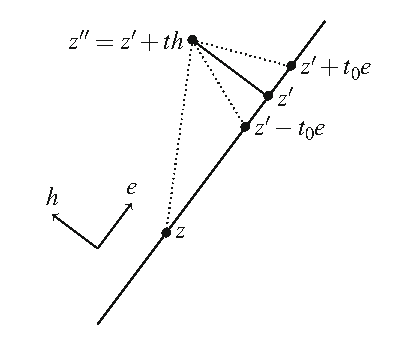
\includegraphics[width=.54\textwidth]{assets/ch03-fig-3-1.pdf}
\caption{\autoref{obj:3.6}证明中使用的点.}\label{fig:3.1}
\end{figure}

\begin{corollary}\label{obj:3.8}
两条不同的传输射线只能相交于同时为二者端点的某个点$z$，且这时$u$在$z$处不可微. 特别地，去掉$u$的不可微点所组成的零测集$\operatorname{Sing}(u)$后，各传输射线互不相交.
\end{corollary}
\begin{proof}
首先注意，如果点$z$属于方向为$e$的传输射线，且$u$在$z$处可微，则必有$e=\nabla u(z)$. 事实上，在$z$附近，对于任意小的$t$（不关心$t$的符号），存在属于同一条射线、形如$z+te$的点；对这些点可以写成
\[
t=u(z+te)-u(z)=\nabla u(z)\cdot te+o(t).
\]
这说明$\nabla u(z)\cdot e=1$. 再结合$|\nabla u(z)|\le1$，唯一可能就是$\nabla u(z)=e$.

现在假设两条传输射线相交于同时为二者内点的点$z$. 这时沿两条射线的方向，$u$在$z$处必须有两个不同的梯度，因而不可能（回顾一下，相交于一点的不同射线必须有不同方向，否则由极大性它们就是同一条射线）.

再假设它们相交于$z$，其中$z$是方向为$e$的一条射线的内点，却是方向$e'\ne e$的另一条射线的端点. 此时$u$在$z$处应可微，而$\nabla u(z)$又必须取两个不同值，同样不可能.

最后，假设交点$z$是两条线段的端点，一条方向为$e$，另一条方向为$e'\ne e$. 如果$u$在$z$处不可微，这时不产生矛盾. 另一方面，若假设$u$在$z$处可微，仍会得到$\nabla u(z)=e=e'$，再次产生矛盾.
\end{proof}

稍后会看到，我们还需要对传输射线的方向作进一步说明.

从本节起，固定一个次级变分问题的最优传输方案$\bar\gamma$，尝试证明它实际上由传输映射诱导. 这里使用$\bar\gamma$实际上集中于某个$c$-CM集合$\Gamma$这一事实（回顾，我们使用的是\eqref{eq:3.3}定义的成本$c$），并考察它与传输射线之间的相互作用. 可以假设$\Gamma\subset A=\{(x,y):u(x)-u(y)=|x-y|\}$，因为任何这样的$\bar\gamma$都必须集中于这一集合，才能使$\int c\,d\bar\gamma$有限. 我们要说明，$\bar\gamma$在每条传输射线上表现为单调递增传输. 更确切地说，有如下结论.

\begin{lemma}\label{obj:3.9}
设$x_1,x_2,y_1,y_2$都在某条传输射线$[x,y]$上，且$(x_1,y_1),(x_2,y_2)\in\Gamma$. 在该射线上通过$x\le x'\iff u(x)\ge u(x')$定义序关系. 则若$x_1<x_2$，就有$y_1\le y_2$.
\end{lemma}
\begin{proof}
由于$\Gamma\subset A$，已知$x_1\le y_1$且$x_2\le y_2$. 因而唯一需要考虑的是$x_1<x_2\le y_2<y_1$的情形. 证明这种情形不可能，就证明了结论. 而这确实不可能，因为$\Gamma$为$c$-CM，且在这一条传输射线上，由所假设的序关系及$u$在该线段上的行为，条件$(x_1,y_2),(x_2,y_1)\in A$成立. 这蕴含$(x_1-x_2)\cdot(y_1-y_2)\ge0$. 但它是两个平行于$e$的向量的标量积，因此在线段上，这正意味着$y_1,y_2$的排序必须与$x_1,x_2$相同.
\end{proof}

由\autoref{sec:2}已见的结果，当$s$为线段，而$\Gamma'\subset s\times s$满足
\[
(x_1,y_1),(x_2,y_2)\in\Gamma',\ x_1<x_2\implies y_1\le y_2
\]
（使用$s$上的序关系）时，$\Gamma'$包含在某个单调递增多值函数的图中，此函数给每一点对应一个点或一条线段. 由于这些线段的内部互不相交，其像不是单点的点至多可数（见\autoref{obj:2.8}的证明）. 这意味着，除去$s$中至多可数的点后，$\Gamma'$包含在$s$上的一个图中. 我们将把这一想法用于$\Gamma'=\Gamma\cap(s\times s)$，其中$s$是传输射线.

概括每条传输射线上的结论，得到：
\begin{proposition}\label{obj:3.10}
最优传输方案$\bar\gamma$集中于一个集合$\Gamma$，具有以下性质：
\begin{itemize}
\item 若$(x,y)\in\Gamma$，则
\begin{itemize}
\item 或者$x\in\operatorname{Sing}(u)$（但该点集为Lebesgue零测集）；
\item 或者$x\notin\operatorname{Trans}(u)$，即它不属于非退化传输射线（此时必有$y=x$，否则$[x,y]$就包含在某条非退化传输射线中）；
\item 或者$x\in\operatorname{Trans}^{(b+)}(u)\setminus\operatorname{Sing}(u)$（此时必有$y=x$，因为$x$属于唯一的传输射线，而由序关系$x\le y$，它的像不可能为$s$中的另一个点）；
\item 或者$x\in\operatorname{Trans}(u)\setminus(\operatorname{Trans}^{(b+)}(u)\cup\operatorname{Sing}(u))$，且$y$属于经过$x$的同一条传输射线（该射线唯一）；
\end{itemize}
\item 在每条传输射线$s$上，$\Gamma\cap(s\times s)$包含于一个单调递增多值函数的图中；
\item 在每条传输射线$s$上，集合
\[
N_s=\{x\in s\setminus\operatorname{Trans}^{(b+)}(u):\#\{y:(x,y)\in\Gamma\}>1\}
\]
可数.
\end{itemize}
显然，若$\mu(\bigcup_sN_s)=0$，即可以去掉每条传输射线上可数个点，则$\bar\gamma$由传输映射诱导.
\end{proposition}

% 以上命题3.10之后续接原PDF121页.
这也可以用测度分解的语言表述（如果$\mu$绝对连续，那么沿各射线$s$分解$\mu$所得的全部测度$\mu_s$都无原子；分解的概念见\autoref{sec:2.3}中的\autoref{box:2.2}），不过为简单起见，我们尽量避免这种论证. 唯一需要的是如下性质（性质N，其中N表示零测性）.

\begin{definition}\label{obj:3.11}
对于给定的Kantorovich势$u$，如果每个满足下列条件的$B\subset\Omega$都有$|B|=0$，则称性质N成立：
\begin{itemize}
\item $B\subset\operatorname{Trans}(u)\setminus\operatorname{Trans}^{(b+)}(u)$；
\item 对每条传输射线$s$，$B\cap s$至多可数.
\end{itemize}
\end{definition}

这一性质并非对$\mathbb R^d$中任意互不相交的线段族都成立. 有一个Alberti、Kirchheim与Preiss构造、后来由Ambrosio、Kirchheim与Pratelli改进的例子（见\cite{b14}）：立方体内的一族互不相交线段，其全部中点的集合却有正测度. 我们将证明传输射线的方向满足额外性质，从而保证性质N.

注意，照例忽略正在构造的传输映射$\mathrm T$的可测性问题：该映射由每条线段上的单调映射粘合而成，但这种粘合应以可测的方式进行\footnote{可以通过限制在一个$\sigma$-紧集$\Gamma$上证明可测性，也可以考虑分解所得的$\mu_s$、$\nu_s$，并使用在每个$s$上$\mathrm T$是把$\mu_s$送到$\nu_s$的单调映射这一事实（因此它继承了$\mu_s$、$\nu_s$关于$s$的依赖关系的某些可测性性质，这些性质由抽象分解定理保证）.}.

证明性质N的主要工具，看来是传输射线方向的Lipschitz正则性（该方向与$\nabla u$的方向相同）.

\begin{theorem}\label{obj:3.12}
如果$\nabla u$为Lipschitz连续，或者存在可数集族$E_h$，使$\nabla u$限制在每个$E_h$上均Lipschitz连续，并且$|\operatorname{Trans}(u)\setminus\bigcup_hE_h|=0$，则性质N成立.
\end{theorem}
\begin{proof}
先假设$\nabla u$为Lipschitz函数. 考虑所有平行于$d-1$个坐标轴、且最后一个坐标为有理数的超平面. 取性质N定义中的集合$B$. 根据定义，$B$中的点属于非退化传输射线，即正长度的线段. 因而$B$中的每一点都属于一条传输射线，该射线与上述至少一个超平面恰交于其内部的一点. 因为这些超平面可数，通过取可数并，可以假设$B$包含在一族全部与同一个超平面$Y$相交的传输射线$S_Y$中. 此外，还可假设$B$不包含同时为两条不同传输射线端点的点，因为已知这些点为零测集. 固定这样的超平面$Y$，考虑如下形式的映射$f:Y\times\mathbb R\to\mathbb R^d$：对$y\in Y$及$t\in\mathbb R$，定义$f(y,t)=y+t\nabla u(y)$. 该映射在我们关心的集合$A\subset Y\times\mathbb R$上良定义且为单射. 集合$A$由满足下列条件的点对$(y,t)$构成：$y$属于$S_Y$中一条传输射线的内部，因而$u$在该点可微，而$y+t\nabla u(y)$属于同一射线的内部. 映射$f$为单射，因为若$(y,t)$与$(y',t')$的像相同，就意味着两条不同传输射线相交于该点. 由构造，$B$包含在$f$的像中，故$f$是$B':=f^{-1}(B)$与$B$之间的双射. 由于$\nabla u$的Lipschitz性质，$f$也Lipschitz连续. 注意，$B'$是$Y\times\mathbb R$的子集，在每条直线$\{y\}\times\mathbb R$上至多含可数个点. 由Fubini定理，这蕴含$|B'|=0$. 因而还有$|B|=|f(B')|\le\operatorname{Lip}(f)^d|B'|$，从而$|B|=0$.

显然，当$\nabla u$并非Lipschitz，但在覆盖$\operatorname{Trans}(u)$几乎所有点的划分的每个集合$E_h$上Lipschitz连续时，结论仍成立：对全部$B\cap E_h$应用同样论证，再取可数并即可（\autoref{fig:3.2}）.
\end{proof}

\begin{figure}[htbp]\centering
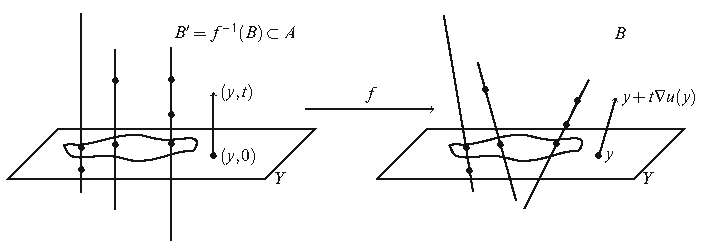
\includegraphics[width=.92\textwidth]{assets/ch03-fig-3-2.pdf}
\caption{\autoref{obj:3.12}中的映射$f$. $B$与$B'$中的点在每条直线上仅有可数个，用实心圆点表示.}\label{fig:3.2}
\end{figure}

现在需要证明$\nabla u$可数Lipschitz.
\begin{definition}\label{obj:3.13}
若存在可数集族$E_h$，使函数$f:\Omega\to\mathbb R^d$在每个$E_h$上Lipschitz连续，且$|\Omega\setminus\bigcup_hE_h|=0$，则称$f$为\emph{可数Lipschitz}（countably Lipschitz）.
\end{definition}
注意，“在集合$E$上Lipschitz连续”和“是某个定义在整个$\mathbb R^d$上的Lipschitz连续函数在$E$上的限制”，实际上是同一性质，这是由Lipschitz延拓定理得到的. 事实上，只要$E\subset X$是度量空间，每个$L$-Lipschitz函数$f:E\to\mathbb R$都能延拓成$X$上的$L$-Lipschitz函数. 这称为Kirszbraun定理，使用\autoref{box:1.5}中的函数$f_k$、取$k\ge L$，就容易得到.

我们希望证明$\nabla u$可数Lipschitz. 首先证明，在一列覆盖几乎所有点的集合上，$u$与某些$\lambda$-凸或$\lambda$-凹函数相同. 为此需要一个定义.
\begin{definition}\label{obj:3.14}
若$x\mapsto f(x)-\frac\lambda2|x|^2$凸，则称$f:\Omega\to\mathbb R$为$\lambda$-凸函数；若$x\mapsto f(x)+\frac\lambda2|x|^2$凹，则称其为$\lambda$-凹函数. 注意，不要求数$\lambda$为正，因此$\lambda>0$时$\lambda$-凸函数严格凸，$\lambda<0$时，它们只要求二阶导数（在存在的地方）有下界. 对某个$\lambda$为$\lambda$-凸（或$\lambda$-凹）的函数，称为\emph{半凸}（semi-convex）（或\emph{半凹}，semi-concave）函数.
\end{definition}

\begin{proposition}\label{obj:3.15}
存在集合$E_h$使得：
\begin{itemize}
\item $\bigcup_hE_h=\operatorname{Trans}(u)\setminus\operatorname{Trans}(u)^{(b+)}$；
\item 在每个$E_h$上，函数$u$是某个$\lambda$-凹函数的限制，其中$\lambda$可依赖$h$.
\end{itemize}
\end{proposition}
\begin{proof}
定义
\[
E_h=\left\{x\in\operatorname{Trans}(u):\exists z\in\operatorname{Trans}(u),\ u(x)-u(z)=|x-z|>\frac1h\right\},
\]
粗略地说，它由传输射线上距该射线上端点至少$1/h$的点构成. 显然$E_h\subset\operatorname{Trans}(u)\setminus\operatorname{Trans}(u)^{(b+)}$. 而且容易得到$\bigcup_hE_h=\operatorname{Trans}(u)\setminus\operatorname{Trans}^{(b+)}(u)$.

固定满足以下性质的函数$c_h:\mathbb R^d\to\mathbb R$：$c_h\in C^2(\mathbb R^d)$、$|\nabla c_h|\le1$、对所有$z\in\mathbb R^d$有$c_h(z)\ge|z|$，并且对所有$z\notin B(0,1/h)$有$c_h(z)=|z|$. 令$\lambda_h:=-\|D^2c_h\|_{L^\infty}$（注意，可将该值取为$-1/h$的阶）. 容易核查，若$x\in E_h$，则
\begin{equation*}
\begin{aligned}
u(x)&=\inf_{y\in\mathbb R^d}|x-y|+u(y)\\
&\le\inf_{y\in\mathbb R^d}c_h(x-y)+u(y)\\
&\le\inf_{y\notin B(x,1/h)}|x-y|+u(y)=u(x),
\end{aligned}
\end{equation*}
其中第一个不等式来自$|z|\le c_h(z)$，第二个来自把范围限制为$y\notin B(x,1/h)$. 最后一个等式由$E_h$的定义得到. 这意味着全部不等式实际上都是等式，且对所有$x\in E_h$，都有$u(x)=u_h(x)$，其中
\[
u_h(x):=\inf_{y\in\mathbb R^d}c_h(x-y)+u(y).
\]
重要的是，$u_h$是$\lambda_h$-凹函数.

下面说明这一点. 对这样选取的$\lambda_h$，显然$c_h$为$\lambda_h$-凹函数. 考虑
\begin{equation*}
\begin{aligned}
u_h(x)+\frac{\lambda_h}2|x|^2
&=\inf_{y\in\mathbb R^d}c_h(x-y)+\frac{\lambda_h}2 2|x|^2+u(y)\\
&=\inf_{y\in\mathbb R^d}c_h(x-y)+\frac{\lambda_h}2|x-y|^2
+\lambda_hx\cdot y-\frac{\lambda_h}2|y|^2+u(y).
\end{aligned}
\end{equation*}
最后这一表达式表明$u_h(x)+\frac{\lambda_h}2|x|^2$关于$x$凹，因为它表示为一族凹函数的下确界（$c_h(x-y)+\frac{\lambda_h}2|x-y|^2$凹，$\lambda_hx\cdot y$线性，其余项关于$x$为常数）. 因而$u_h(x)$为$\lambda_h$-凹函数.
\end{proof}

前一定理允许用正则性更好的函数$u_h$替换$u$（因为它们$\lambda$-凹，具有与凸函数相同的正则性）. 可惜这还不够，因为一般凸函数甚至未必可微. 还需要新的可数分解，可以从下面这条不予证明的定理得到.

\begin{theorem}\label{obj:3.16}
若$f$为凸函数，则$\nabla f$可数Lipschitz.
\end{theorem}
该定理的证明见\cite{b13}定理5.34. 当把$\nabla f$换成任意BV函数时，它仍成立，而\cite{b13}正是在这一框架下表述的.

\begin{sourcebox}{知识回顾：$\mathbb R^d$中的BV函数}\label{box:3.1}
在区域$\Omega\subset\mathbb R^d$上，如果$L^1$函数$f:\Omega\to\mathbb R$的分布导数是有限测度，则称它为BV函数. 这意味着要求对每个$C_c^1$向量场$\xi:\Omega\to\mathbb R^d$都有
\[
\int_\Omega f(\nabla\cdot\xi)\,dx\le C\|\xi\|_{L^\infty}.
\]
因此BV空间比Sobolev空间$W^{1,p}$更宽，后者要求分布导数属于$L^p$（即它们为具有可积性性质的绝对连续测度）.

分布导数$\nabla f$并非任意测度，而必须形如$\nabla f=\nabla^af(x)\,dx+D^sf+D^jf$，其中$\nabla^af(x)\,dx$是$\nabla f$关于Lebesgue测度的绝对连续部分，$D^jf$是所谓跳跃部分，关于$\mathscr H^{d-1}$有密度（它集中于点集$J_f$，在每个这样的点上，存在一个超平面，使函数$f$在超平面两侧有两个不同极限，取适当的测度论意义；而$D^ju$关于$\mathscr H^{d-1}_{|J_f}$的密度恰好是这两个极限值之差乘以超平面的法向方向：$D^jf=(f^+-f^-)n_{J_f}\cdot\mathscr H^{d-1}_{|J_f}$），$D^c$则为所谓Cantor部分，它与Lebesgue测度奇异，但在任意$(d-1)$维集合上为零.

以$BV_{\mathrm{loc}}(\mathbb R^d)$表示局部BV函数空间，即其导数为Radon测度、也就是局部有限测度的函数（在使用检验函数$\xi$的定义中，取$\xi\in C_c^1(\mathbb R^d)$，常数$C$可以依赖$\xi$的支集）. 向量值BV函数就是逐分量为BV的函数$f=(f_1,\ldots,f_k):\mathbb R^d\to\mathbb R^k$，即对每个$i=1,\ldots,k$都有$f_i\in BV$. 有意思的是，凸函数的梯度$g=\nabla f$总是局部BV的. 这是因为凸函数梯度的Jacobian矩阵就是该函数的Hessian矩阵，并且正定. 这意味着矩阵值分布$\nabla(\nabla f)=D^2f$为正分布，而正分布必定为正测度（注意：涉及矩阵值和向量值函数时，这需要精确定义）.

BV函数关于Lebesgue或$\mathscr H^{d-1}$测度几乎处处满足多种精细正则性，读者可参见\cite{b13,b160}. 特别引用如下结果（它绝非容易的结果），由它可以推出\autoref{obj:3.16}.
\begin{theorem*}
若$f\in BV_{\mathrm{loc}}(\mathbb R^d)$，则$f$可数Lipschitz.
\end{theorem*}
\end{sourcebox}

由\autoref{obj:3.15}及\autoref{obj:3.16}得到：
\begin{proposition}\label{obj:3.17}
若$u$是Kantorovich势，则$\nabla u:\operatorname{Trans}(u)\to\mathbb R^d$可数Lipschitz.
\end{proposition}
\begin{proof}
显然，\autoref{obj:3.16}中的可数Lipschitz正则性也适用于$\lambda$-凸与$\lambda$-凹函数的梯度. 这意味着$\nabla u_h$具有这一性质，再取可数并，$\nabla u$也具有该性质.
\end{proof}

\subsubsection{最优传输映射的存在与不存在}\label{sec:3.1.4}
由前面各节的分析，得到下面主要取自\cite{b10,b14,b44}的结果.
\begin{theorem}\label{obj:3.18}
在通常假设$\mu\ll\mathscr L^d$下，次级变分问题存在唯一解$\bar\gamma$，它由传输映射$\mathrm T$诱导，并在每条传输射线上单调非减.
\end{theorem}
\begin{proof}
\autoref{obj:3.17}与\autoref{obj:3.12}保证性质N成立. 因而可以应用\autoref{obj:3.10}得到$\bar\gamma=\gamma_{\mathrm T}$. 唯一性由通常论证得到：若两个方案$\gamma'=\gamma_{\mathrm T'}$、$\gamma''=\gamma_{\mathrm T''}$都使次级变分问题最优，那么$\frac12\gamma_{\mathrm T'}+\frac12\gamma_{\mathrm T''}$也应如此. 但要使这个测度由映射诱导，必须有$\mathrm T'=\mathrm T''$几乎处处成立（见\autoref{obj:1.19}）.
\end{proof}

\begin{definition}\label{obj:3.19}
最优传输方案$\bar\gamma$称为\emph{沿射线单调的传输方案}（ray-monotone transport plan），相应的传输映射称为\emph{沿射线单调的传输映射}.
\end{definition}
注意，这一分析还附带给出$|\operatorname{Trans}(u)^{(b)}|=0$，因为$\operatorname{Trans}(u)^{(b)}$与每条传输射线相交于两个点，因而由性质N为零测集. 但此前无法证明这一点，所以任何基于分解$\operatorname{Trans}(u)^{(i)}$的策略都还不完整.

为完成本节，还可以问：这一存在性结果真的需要$\mu\ll\mathscr L^d$吗？能否像二次情形那样，用“对每个$(d-1)$-可求长集合$A$都有$\mu(A)=0$”（或\autoref{sec:1.3.1}中的其他条件）保证最优映射存在？

答案是否定的，下面的例子将说明这一点.
\subsubsection*{从图像到正方形的传输}
考虑连续函数$B:[0,1]\to\mathbb R$，满足：对每个Lipschitz函数$f:\mathbb R\to\mathbb R$，集合$\{t\in[0,1]:B(t)=f(t)\}$和$\{t\in[0,1]:f(B(t))=t\}$都是Lebesgue零测集. 取$\mu=(\mathrm{id},B)_\#(\mathscr L^1\restr[0,1])$、$\nu=\mathscr L^2\restr Q$，其中$Q=[0,1]\times[L,L+1]$为正方形，$L=\|B\|_{L^\infty}$.

实际上，$\mu$集中于$B$的图像，$\nu$集中于图像上方的正方形. 这样选取后，测度$\mu$对任意形如$\{(t,f(t))\}$或$\{(f(s),s)\}$的可求长曲线都赋予零质量，其中$f$为Lipschitz函数. 另一方面，它不绝对连续，因为它给一个$\mathscr L^2$-零测的图像赋予正质量. 现在要证明，不存在从$\mu$到$\nu$的最优传输映射（\autoref{fig:3.3}）.

\begin{figure}[htbp]\centering
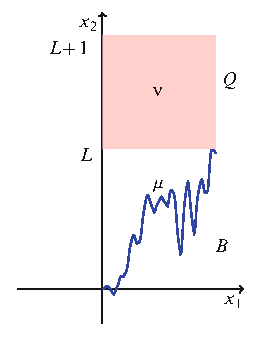
\includegraphics[width=.48\textwidth]{assets/ch03-fig-3-3.pdf}
\caption{测度$\mu$集中于一个图像，$\nu$集中于一个正方形.}\label{fig:3.3}
\end{figure}

首先注意，存在一个显然的传输映射$S$把$\nu$送到$\mu$：只需取$S(x_1,x_2)=(x_1,B(x_1))$（即每一点竖直移到$B$的图像上的相应点）. 显然，$S$不是单射. $S$的Monge成本为$\int_Q|x_2-B(x_1)|\,dx_1dx_2=\int_Q(x_2-B(x_1))\,dx_1dx_2$. 此外，函数$u(x_1,x_2)=-x_2$属于$\operatorname{Lip}_1$，并且
\begin{equation*}
\begin{aligned}
\int_{\mathbb R^2}u\,d(\mu-\nu)
&=-\int_0^1B(x_1)\,dx_1+\int_Qx_2\,dx_1dx_2\\
&=\int_Q|x_2-B(x_1)|\,dx_1dx_2.
\end{aligned}
\end{equation*}
这证明$S$是从$\nu$到$\mu$的最优映射，而$u$为Kantorovich势（更确切地说，$u$是从$\mu$到$\nu$的Kantorovich势，$-u$是从$\nu$到$\mu$的Kantorovich势）. 但这也证明，$\mu$与$\nu$之间任意最优传输方案都必须集中于集合$\{(x,y):y_2-x_2=|x-y|\}$，即$\{(x,y):y_1=x_1,\ x_2\le y_2\}$. 特别地，传输只能竖直发生，恰如$S$那样. 然而，不存在具有这一性质的从$\mu$到$\nu$的传输映射：事实上，$\operatorname{spt}(\mu)$经这种映射得到的像，在$\operatorname{spt}(\nu)$的每条竖直线段上只能含一个点，因而不可能覆盖几乎整个$Q$.

为使例子完整\footnote{注意，这一构造与\cite{b199}中为另一个目的给出的例子本质相同. 正则性程度稍有不同；为使介绍自足，我们决定直接处理“竖直”的Lipschitz曲线.}，只需构造这样的函数$B$. 读者或许已经猜到，记号的选取是有意的：Brown运动的典型轨道满足这一假设. 事实上，已知Brown运动的轨道几乎必然处处不可微，甚至处处不可近似微分（这一概念见\autoref{sec:3.3.2}中的\autoref{box:3.3}；Brown运动在此方面的性质见\cite{b222}）. 顺便说，\cite{b25}还证明，几乎必然不存在维数大于$1/2$的集合$A$，使得$B$在$A$上以大于$1/2$的指数Hölder连续. 因而$B$不可能在一个一维集合上与某个Lipschitz函数相同. 甚至可以说，$\{t\in[0,1]:B(t)=f(t)\}$的维数不大于$1/2$.

另一个集合（即满足$t=f(B(t))$的点）更棘手. 反设存在紧集$K$，满足$|K|>0$且在$K$上$f\circ B=\mathrm{id}$. 则集合$H=B(K)$也紧，并且必须有正测度. 否则，若$|H|=0$，则由于$f$为Lipschitz函数，$K\subset f(H)$也为零测集. 限制$H$后，可以假设$f$为$C^1$函数. 事实上，对每个Lipschitz函数$f$及每个$n$，存在$C^1$函数$\widetilde f_n$使$|\{f\ne\widetilde f_n\}|<1/n$（这一事实见\cite{b160}）. 若令$H_n=\{f=\widetilde f_n\}$，则$|H\setminus\bigcup_nH_n|=0$且$|f(H\setminus\bigcup_nH_n)|=0$；这证明$|f(\bigcup_nH_n)|=|\bigcup_nf(H_n)|>0$，因而至少对某个$n$，必须有$|H_n|,|f(H_n)|>0$. 所以可以假设$f\in C^1$. 现在有两种可能：或者$f'=0$在$H$上成立，或者存在一个小区间，$f$在其上为微分同胚. 后一种情形下，在正测度集合上有$B=f^{-1}$，与Brown运动的已知性质矛盾（因为$f^{-1}$为Lipschitz函数，甚至为$C^1$函数）. 相反，若$f'=0$在$H$上成立，则面积公式给出$|K|=0$，同样矛盾.

\subsubsection{沿射线单调最优传输的逼近问题}\label{sec:3.1.5}
本节讨论关于沿射线单调最优传输方案$\bar\gamma$的一些自然问题，特别是逼近问题. 事实上，已经看到（\autoref{obj:1.50}），对于任意弱收敛序列$\gamma_n\rightharpoonup\gamma$，如果$\gamma_n$对于某个连续成本在其边缘测度之间最优，则$\gamma$也是最优的. 但我们知道，对于$c(x,y)=|x-y|$，最优传输方案一般不唯一，而在许多应用中，人们希望选用沿射线单调的那个. 因此，问题是：当测度和／或成本变化时，怎样通过逼近选取这一特殊方案？

在许多应用中（尤其见\autoref{sec:4}），用把给定测度送到原子测度的传输映射来逼近传输方案很有意义，因为这类映射实际上由区域划分上定义的不同位似组成.

下面给出一个有用的逼近引理，其思路类似$\Gamma$-收敛展开（见\cite{b77}第2.4节，以及\autoref{sec:4.4.2}中的\autoref{box:4.6}）.

对固定测度$\mu,\nu\in\mathscr P(\Omega)$且$\mu\ll\mathscr L^d$，考虑下列极小化问题族$(P_\varepsilon)$：
\begin{equation*}
\begin{aligned}
(P_\varepsilon)=\min\bigl\{&\mathscr T_c((\pi_y)_\#\gamma,\nu)+\varepsilon K_1(\gamma)+\varepsilon^2K_2(\gamma)
+\varepsilon^{3d+3}\#((\pi_y)_\#\gamma):\\
&\gamma\in\mathscr P(\Omega\times\Omega),\ (\pi_x)_\#\gamma=\mu\bigr\},
\end{aligned}
\end{equation*}
其中$\mathscr T_c$为成本$c(x,y)=|x-y|$的传输问题最小值，$K_p(\gamma)=\int|x-y|^p\gamma(dx,dy)$，$p=1,2$，符号$\#$表示测度支集的基数. 注意，一般有$K_1(\gamma)\ne\mathscr T_c((\pi_x)_\#\gamma,(\pi_y)_\#\gamma)$.

实际上，极小化$(P_\varepsilon)$就是寻找第一边缘测度为$\mu$的传输方案，按重要性递减的顺序满足以下标准：第二边缘测度应接近$\nu$；传输的$K_1$成本应小；$K_2$成本也应小；最后，第二边缘测度必须是原子的，且原子数不太多.

这个极小化问题显然至少有一个解（由直接法，因为$\Omega$紧）. 以$\gamma_\varepsilon$表示一个这样的解，$\nu_\varepsilon:=(\pi_y)_\#\gamma_\varepsilon$为其第二边缘测度. 显然$\nu_\varepsilon$为原子测度，$\gamma_\varepsilon$是$\min\{K_1(\gamma)+\varepsilon K_2(\gamma):\gamma\in\Pi(\mu,\nu_\varepsilon)\}$的解（由于$\mu\ll\mathscr L^d$，此解唯一）；该问题正是从$\mu$到$\nu_\varepsilon$、成本为$|x-y|+\varepsilon|x-y|^2$的最优传输问题. 令
\begin{equation}\label{eq:3.4}
\bar\gamma=\operatorname*{argmin}\{K_2(\gamma):\gamma\text{ 是从 }\mu\text{ 到 }\nu\text{ 的 }K_1\text{-最优传输方案}\}.
\end{equation}
该传输方案$\bar\gamma$唯一，也是从$\mu$到$\nu$的唯一沿射线单调最优传输方案（由\autoref{sec:3.1.4}得到）；注意，泛函$K_2$可以替换为任意$\gamma\mapsto\int h(x-y)\,d\gamma$，其中$h$严格凸.

\begin{lemma}\label{obj:3.20}
当$\varepsilon\to0$时，$\nu_\varepsilon\rightharpoonup\nu$且$\gamma_\varepsilon\rightharpoonup\bar\gamma$.
\end{lemma}
\begin{proof}
只需证明，任何子列的可能极限分别等于$\nu$或$\bar\gamma$. 令$\gamma_0$为一个这样的极限，$\nu_0=(\pi_y)_\#\gamma_0$为相应$\nu_\varepsilon$子列的极限. 考虑由大约$Cn^d$个点构成的规则网格$G_n\subset\Omega$（取$G_n=\frac1n\mathbb Z^d\cap\Omega$），并令$p_n$为从$\Omega$到$G_n$的任意可测映射，满足$|p_n(x)-x|\le1/n$（例如，在定义良好处可以取投影映射）. 令$\nu^n=(p_n)_\#\nu$，注意$\#\nu^n\le Cn^d$，$\nu^n\rightharpoonup\nu$，且$\mathscr T_c(\nu^n,\nu)\le1/n$.

\emph{第一步：$\nu_0=\nu$.} 取从$\mu$到$\nu^n$的任意传输方案$\gamma^n$. 由$\gamma_\varepsilon$的最优性，
\[
\mathscr T_c(\nu_\varepsilon,\nu)\le\mathscr T_c(\nu^n,\nu)+\varepsilon K_1(\gamma^n)
+\varepsilon^2K_2(\gamma^n)+C\varepsilon^{3d+3}n^d.
\]
固定$n$，令$\varepsilon\to0$，得到
\[
\mathscr T_c(\nu_0,\nu)\le\mathscr T_c(\nu^n,\nu)\le\frac1n.
\]
再令$n\to\infty$，得到$\mathscr T_c(\nu_0,\nu)=0$，从而$\nu_0=\nu$（由\autoref{obj:3.3}）.

\emph{第二步：$\gamma_0$对于$K_1$是从$\mu$到$\nu$的最优方案.} 取从$\mu$到$\nu^n$的任意最优传输方案$\gamma^n$（成本为$K_1$，即$K_1(\gamma^n)=\mathscr T_c(\mu,\nu^n)$）. 这些方案收敛于从$\mu$到$\nu$的某个最优方案$\widetilde\gamma$（即$K_1(\widetilde\gamma)=\mathscr T_c(\mu,\nu)$）. 由$\gamma_\varepsilon$的最优性，有
\begin{equation*}
\begin{aligned}
\varepsilon K_1(\gamma_\varepsilon)
&\le\mathscr T_c(\nu^n,\nu)+\varepsilon K_1(\gamma^n)+\varepsilon^2K_2(\gamma^n)+C\varepsilon^{3d+3}n^d\\
&\le\frac1n+\varepsilon K_1(\gamma^n)+C\varepsilon^2+C\varepsilon^{3d+3}n^d.
\end{aligned}
\end{equation*}
取$n\approx\varepsilon^{-2}$并除以$\varepsilon$，得到
\[
K_1(\gamma_\varepsilon)\le\varepsilon+K_1(\gamma^n)+C\varepsilon+C\varepsilon^{d+2}.
\]
取极限得到
\[
K_1(\gamma_0)\le K_1(\widetilde\gamma)=\mathscr T_c(\mu,\nu),
\]
从而$\gamma_0$也最优.

\emph{第三步：$\gamma_0=\bar\gamma$.} 取从$\mu$到$\nu$、成本$K_1$的任意最优传输方案$\gamma$. 令$\gamma^n=(\mathrm{id}\times p_n)_\#\gamma$，其中$(\mathrm{id}\times p_n)(x,y):=(x,p_n(y))$. 有$(\pi_y)_\#\gamma^n=\nu^n$，因而
\begin{equation*}
\begin{aligned}
\mathscr T_c(\nu_\varepsilon,\nu)+\varepsilon K_1(\gamma_\varepsilon)+\varepsilon^2K_2(\gamma_\varepsilon)
&\le\mathscr T_c(\nu^n,\nu)+\varepsilon K_1(\gamma^n)\\
&\quad+\varepsilon^2K_2(\gamma^n)+C\varepsilon^{3d+3}n^d.
\end{aligned}
\end{equation*}
此外，使用\autoref{obj:3.2}的三角不等式，推出
\[
K_1(\gamma_\varepsilon)\ge\mathscr T_c(\mu,\nu_\varepsilon)
\ge\mathscr T_c(\mu,\nu)-\mathscr T_c(\nu_\varepsilon,\nu).
\]
还有
\begin{equation*}
\begin{aligned}
K_1(\gamma^n)&\le K_1(\gamma)+\int|p_n(y)-y|\,d\gamma(x,y)\\
&\le K_1(\gamma)+\frac1n=\mathscr T_c(\mu,\nu)+\frac1n.
\end{aligned}
\end{equation*}
因而有
\begin{equation*}
\begin{aligned}
&(1-\varepsilon)\mathscr T_c(\nu_\varepsilon,\nu)+\varepsilon\mathscr T_c(\mu,\nu)+\varepsilon^2K_2(\gamma_\varepsilon)\\
&\qquad\le\frac1n+\varepsilon\mathscr T_c(\mu,\nu)+\frac\varepsilon n
+\varepsilon^2K_2(\gamma^n)+C\varepsilon^{3d+3}n^d.
\end{aligned}
\end{equation*}
去掉左侧第一项（它为正），消去$\varepsilon\mathscr T_c(\mu,\nu)$，再除以$\varepsilon^2$，得到
\[
K_2(\gamma_\varepsilon)\le\frac{1+\varepsilon}{n\varepsilon^2}+K_2(\gamma^n)+C\varepsilon^{3d+1}n^d.
\]
这里只需取$n\approx\varepsilon^{-3}$并取极限，即得
\[
K_2(\gamma_0)\le K_2(\gamma),
\]
这正是刻画$\bar\gamma$的条件（在$K_1$极小元之中$K_2$最优）.
\end{proof}

这一逼近结果将用于\autoref{sec:4}. 它主要基于\autoref{sec:3.1.2}中已经提到的事实：极小化传输成本$|x-y|+\varepsilon|x-y|^2$时，会收敛于次级变分问题的解，即沿射线单调的传输映射. 如前所说，任意严格凸扰动应当起到与二次扰动相同的作用.

不过，还有其他同样自然的逼近，至今仍是开放问题. 下面列出两个.
\begin{openproblem}[单调传输的稳定性]
令$\gamma_n$为成本$|x-y|$下$\mu_n$与$\nu_n$之间沿射线单调的最优传输方案. 假设$\mu_n\rightharpoonup\mu$、$\nu_n\rightharpoonup\nu$、$\gamma_n\rightharpoonup\gamma$. $\gamma$是否为$\mu$与$\nu$之间沿射线单调的最优传输方案？
\end{openproblem}
\begin{openproblem}[正则化距离成本的极限]
令$\gamma_\varepsilon$为两个给定测度$\mu$、$\nu$之间成本$\sqrt{\varepsilon^2+|x-y|^2}$的最优传输方案. 若$\operatorname{spt}(\mu)\cap\operatorname{spt}(\nu)=\varnothing$，则容易证明$\gamma_\varepsilon$收敛于沿射线单调的最优传输方案（因为按$\varepsilon$的首个非零阶，成本扰动形如$|x-y|+\varepsilon^2/|x-y|+o(\varepsilon^2)$，且函数$h(t)=1/t$在$\{t>0\}$上严格凸）. 若两测度的支集相交（或相同），同一结论是否仍成立？
\end{openproblem}
最后这一逼近在证明（或尝试证明）正则性结果时很有用（见\cite{b210}）.
